\documentclass[letterpaper,final,12pt,reqno]{amsart}

\usepackage[total={6.3in,9.2in},top=1.1in,left=1.1in]{geometry}

\usepackage{times,bm,bbm,empheq,fancyvrb,graphicx,amsthm,amssymb}
\usepackage[dvipsnames]{xcolor}
\usepackage{longtable}
\usepackage{booktabs}

\usepackage{tabto}
\TabPositions{1.5cm}

\usepackage{tikz}
\usetikzlibrary{decorations.pathreplacing}

\usepackage[kw]{pseudo}
\pseudoset{%
left-margin=15mm,%
topsep=5mm,%
label=\footnotesize\arabic*,%
idfont=\texttt,%
ctfont=\textsl,%
ct-left=\qquad\qquad(,%
ct-right=),%
}

\usepackage{float}

% hyperref should be the last package we load
\usepackage[pdftex,
colorlinks=true,
plainpages=false, % only if colorlinks=true
linkcolor=blue,   % ...
citecolor=Red,    % ...
urlcolor=black    % ...
]{hyperref}

\renewcommand{\baselinestretch}{1.05}

\allowdisplaybreaks[1]  % allow display breaks in align environments, if they avoid major underfulls

\newtheoremstyle{cstyle}% name
  {5pt}% space above
  {5pt}% space below
  {\itshape}% body font
  {}% indent amount
  {\itshape}% theorem head font
  {.}% punctuation after theorem head
  {.5em}% space after theorem head
  {\thmname{#1}\thmnumber{ #2}\thmnote{ (#3)}}% theorem head spec
\theoremstyle{cstyle}

\newtheorem{theorem}{Theorem}
\newtheorem{lemma}[theorem]{Lemma}
\newtheorem{assumptions}[theorem]{Assumptions}

\newtheoremstyle{cstyle*}% name
  {5pt}% space above
  {5pt}% space below
  {\itshape}% body font
  {}% indent amount
  {\itshape}% theorem head font
  {.}% punctuation after theorem head
  {.5em}% space after theorem head
  {\thmname{#1}}% theorem head spec
\theoremstyle{cstyle*}
\newtheorem{assumptions*}{Assumptions}

\newtheoremstyle{dstyle}% name
  {5pt}% space above
  {5pt}% space below
  {}%{\itshape}% body font
  {}% indent amount
  {\itshape}% theorem head font
  {.}% punctuation after theorem head
  {.5em}% space after theorem head
  {\thmname{#1}\thmnumber{ #2}\thmnote{ (#3)}}% theorem head spec
\theoremstyle{dstyle}

\newtheorem{definition}[theorem]{Definition}
\newtheorem{example}[theorem]{Example}

% numbering
\numberwithin{equation}{section}
\numberwithin{figure}{section}
\numberwithin{table}{section}
\numberwithin{theorem}{section}

\newcommand{\eps}{\epsilon}
\newcommand{\RR}{\mathbb{R}}

\newcommand{\grad}{\nabla}
\newcommand{\Div}{\nabla\cdot}
\newcommand{\trace}{\operatorname{tr}}

\newcommand{\hbn}{\hat{\mathbf{n}}}

\newcommand{\bb}{\mathbf{b}}
\newcommand{\be}{\mathbf{e}}
\newcommand{\bbf}{\mathbf{f}}
\newcommand{\bg}{\mathbf{g}}
\newcommand{\bn}{\mathbf{n}}
\newcommand{\br}{\mathbf{r}}
\newcommand{\bu}{\mathbf{u}}
\newcommand{\bv}{\mathbf{v}}
\newcommand{\bw}{\mathbf{w}}
\newcommand{\bx}{\mathbf{x}}
\newcommand{\bF}{\mathbf{F}}
\newcommand{\bV}{\mathbf{V}}
\newcommand{\bX}{\mathbf{X}}
\newcommand{\bxi}{\bm{\xi}}
\newcommand{\bzero}{\bm{0}}

\newcommand{\cK}{\mathcal{K}}
\newcommand{\cV}{\mathcal{V}}

\newcommand{\rhoi}{\rho_{\text{i}}}

\newcommand{\ip}[2]{\left<#1,#2\right>}

\newcommand{\mR}{R^{\bm{\oplus}}}
\newcommand{\iR}{R^{\bullet}}

\newcommand{\nn}{{\text{n}}}
\newcommand{\pp}{{\text{p}}}
\newcommand{\qq}{{\text{q}}}
\newcommand{\rr}{{\text{r}}}

\newcommand{\supp}{\operatorname{supp}}
\newcommand{\Span}{\operatorname{span}}


\begin{document}
\title[On multilevel constraint decomposition methods]{On multilevel constraint decomposition methods \\ for nonlinear variational inequalities}

\author{Ed Bueler}

\date{\today}

\begin{abstract} FIXME
\end{abstract}

\maketitle

%\tableofcontents

\thispagestyle{empty}
%\bigskip

\newfloat{pseudofloat}{t}{xyz}[section]
\floatname{pseudofloat}{Algorithm}


\section{Introduction} \label{sec:intro}

The goal of this paper is to extend the constraint decomposition (CD) method of X.-C.~Tai \cite{Tai2003} to nonlinear variational inequality (VI) problems, such as obstacle problems, to which it has not been applied.  The convergence of this method, for several types of decompositions, was proven by Tai for coercive VI problems which arise from minimization of a convex functional over a convex set.  In its multilevel form the method has been shown to have optimal complexity for elliptic, linear obstacle problems \cite[Subsection 5.4]{Tai2003}; see also \cite[Theorem 4.6 and Algorithm 4.7]{GraeserKornhuber2009}.

The theory presented in \cite{Tai2003} is extended in three particular directions:
\renewcommand{\labelenumi}{\emph{(\roman{enumi})}}
\begin{enumerate}
\item We do not assume that the continuum VI problem arises from optimization of a scalar objective---examples are explored in Sections \ref{sec:vi} and \ref{sec:results}---but we prove convergence in $H^1$ norm at the same rate as the original method converges in energy (Section \ref{sec:convergence}). % THIS IS THE HOPE

\item We make finite element (FE) implementations of the multilevel CD algorithm more practical by addressing storage of intermediate quantities.  Specifically, in Section \ref{sec:results} we show results from a full approximation storage (FAS; see \cite{Brandt1977,Bruneetal2015}) implementation for nonlinear operators, one which avoids global (Newton) linearization; compare \cite{GraeserKornhuber2009}.

\item We observe that multilevel ``up-smoothing'' is intrinsically more efficient than ``down-smoothing'' (Section \ref{sec:multilevel}).  This observation seems to be new; compare the comments on V(1,0) and V(1,1) cycles in \cite{GraeserKornhuber2009,Tai2003}.  A strong preference for up-smoothing is special to multilevel CD methods and does not arise in unconstrained problems.
\end{enumerate}

For problems of porous-media type the nonlinear operator $f$ is not known to be coercive, so the convergence theory in \emph{(i)} does not apply.  However, a full-cycle implementation of the multilevel CD method is demonstrated numerically.  By ``freezing' the solution-dependent coefficient, the operator is approximated by a coercive operator, nonlinear in general, for the duration of the V-cycle.  The resulting scheme is highly-effective for doubly-nonlinear diffusion operators (Section \ref{sec:results}).

For the classical obstacle problem with a Laplacian operator, certain multilevel techniques are known to improve performance relative to the multilevel CD method \cite{GraeserKornhuber2009}.  These improved methods either track the active set in the discretization or modify the nodal basis functions, and in this sense they are discrete algorithms.  By contrast the CD method applies at the level of the continuum problem (Sections \ref{sec:cd} and \ref{sec:convergence}); compare the truncated monotone multigrid method \cite{Kornhuber1994}, for example.  Acceleration of our nonlinear multilevel CD method via active-set and/or basis-level manipulations represents a potential extension of the method here, and is a topic for future research.

The iterates from a CD method are always admissible, and thus the operator need only be defined for admissible states; Section \ref{sec:results} includes a nontrivial example.  Admissible-iterate methods should permit direct solutions of certain VI problems, such as fluid-layer dynamics problems \cite{Bueler2021conservation,JouvetBueler2012}, for which non-admissible methods, such as semi-smooth methods \cite{BensonMunson2006}, require unnatural modifications of the operator formula.  The full-cycle scheme in \emph{(ii)} above is also designed for these problems, which are characterized by the solution of an auxiliary PDE on a domain determined inside the VI residual evaluation.

% A BRIDGE TOO FAR:  In one example at the end of this paper (Section \ref{sec:resultsnonlocal}) we consider a nonlocal residual functional, that is, one which is not a partial differential operator.  Each evaluation of this functional requires the solution of a Stokes problem for a layer of fluid \nocite{SayagWorster2013} on a substrate (which forms the obstacle), and thus the corresponding FE operator discretization is also not sparse.  In this case we cannot prove coercivity but we nonetheless succeed in demonstrating near-optimal complexity of the Section \ref{sec:multilevel} multilevel CD algorithm in practice.


\section{Coercive variational inequalities} \label{sec:vi}

Suppose $\cV$ is a real, reflexive Banach space with norm $\|\cdot\|$ and topological dual space $\cV'$.  Denote the dual pairing of $\phi \in \cV'$ and $v\in\cV$ by $\ip{\phi}{v} = \phi(v)$, and note that $\|\phi\|_{\cV'} = \sup_{\|v\|=1} |\ip{\phi}{v}|$ defines a (Banach space) norm on $\cV'$.  Let $\cK \subset \cV$ be a nonempty closed and convex subset, the \emph{constraint set}; elements of $\cK$ are said to be \emph{admissible}.

For a continuous, but generally nonlinear, operator $f:\cK \to \cV'$ and a linear \emph{source functional} $\ell\in \cV'$ we consider the following \emph{variational inequality} (VI) for the (exact) solution $u^*\in \cK$, if it exists:
\begin{equation}
\ip{f(u^*)}{v-u^*} \ge \ip{\ell}{v-u^*} \qquad \text{for all } v\in \cK. \label{eq:vi}
\end{equation}
Because $f$ is (generally) nonlinear, the source term $\ell$ is not strictly needed for posing this VI,\footnote{By redefining $f$ we may take $\ell=0$.} but its presence is helpful to algorithms in Section \ref{sec:multilevel}.

VI \eqref{eq:vi} generalizes the nonlinear system of equations $f(u^*)=\ell$ to the constraint set $\cK$.  Informally, if we conceptualize the dual pairing as an inner product then \eqref{eq:vi} says that the angle between $f(u^*)-\ell$ and any arbitrary vector $v-u$ pointing from $u$ into $\cK$ is at most $90^\circ$.  That is, \eqref{eq:vi} says that $f(u^*)-\ell$ may not be zero but it points directly into $\cK$.  However, if $u^*$ is in the interior $\cK^\circ$ then \eqref{eq:vi} implies $f(u^*)=\ell$.

\begin{definition} The following definitions are standard \cite{KinderlehrerStampacchia1980}.  A map $f:\cK \to \cV'$ is \emph{monotone} if
\begin{equation}
\ip{f(u)-f(v)}{u-v} \ge 0 \qquad \text{for all } u,v \in \cK, \label{eq:monotone}
\end{equation}
\emph{strictly monotone} if equality in \eqref{eq:monotone} implies $u=v$, and \emph{coercive} if there exists $w \in \cK$ so that
\begin{equation}
\frac{\ip{f(u)-f(w)}{u-w}}{\|u-w\|} \to +\infty \qquad \text{as } \|u\|\to +\infty. \label{eq:coercive}
\end{equation}
We say VI \eqref{eq:vi} is \emph{monotone} if $f$ is monotone, and likewise for strictly monotone and coercive. \end{definition}

It is well-known that if $f:\cK \to \cV'$ is continuous, monotone, and coercive then VI \eqref{eq:vi} has a solution \cite[Corollary III.1.8]{KinderlehrerStampacchia1980}, and also that the solution $u^* \in \cK$ is unique when $f$ is strictly monotone.  As in the calculus of variations \cite{Evans2010}, coercivity permits a compactness argument for unbounded sets $\cK$; recall that the bounded, closed subsets of a reflexive Banach space are weakly compact.  The condition of continuity can be weakened to only apply on finite-dimensional subspaces \cite{KinderlehrerStampacchia1980}, but the stronger condition will apply in our examples.

The coercive VIs solved in this paper satisfy a stronger inequality than \eqref{eq:coercive}, and thus they are well-posed.

\begin{definition}  Let $p>1$.  The map $f:\cK \to \cV'$ is \emph{$p$-coercive} if there exists $\kappa>0$ such that
\begin{equation}
\ip{f(u)-f(v)}{u-v} \ge \kappa \|u-v\|^p \qquad \text{for all } u,v \in \cK. \label{eq:pcoercive}
\end{equation}
\end{definition}

It is easy to see that if $f$ is $p$-coercive then it is monotone, strictly monotone, and coercive.  Note that Tai \cite{Tai2003} uses ``coercive'' for what we call $2$-coercive.  The following result holds.

\begin{theorem}  \label{thm:viwellposed}  If $f:\cK \to \cV'$ is continuous and $p$-coercive then there exists a unique $u^*\in \cK$ solving VI \eqref{eq:vi}.
\end{theorem}

When $f$ is monotone, \eqref{eq:vi} generalizes the problem of minimizing a convex function over $\cK$.  In fact, suppose $F:\cK \to \RR$ is lower semi-continuous and (G\^ateau) differentiable with continuous derivative $F':\cK \to \cV'$.  Then $F$ is convex if and only if $F'$ is monotone \cite[Proposition I.5.5]{EkelandTemam1976}.  Furthermore, Proposition II.2.1 in \cite{EkelandTemam1976} shows that if $F$ is convex then \eqref{eq:vi} holds for $f=F'$ and $\ell=0$ if and only if
\begin{equation}
u^* = \operatorname{arg-min}_{v\in\cK} F(v). \label{eq:minimization}
\end{equation}
The CD methods of Tai \cite{Tai2003} address problem \eqref{eq:minimization} under the hypothesis that $F'$ is 2-coercive.

From now on $\Omega \subset \RR^d$ denotes a bounded, open set with smooth or piecewise-smooth (e.g.~polygonal) boundary.  Sobolev spaces \cite{Evans2010} are denoted by $W^{k,p}(\Omega)$, for integer $k$ and $1\le p \le \infty$, with $W^{k,2}$ denoted $H^k$.  The following example includes the classical obstacle problem for the linear Laplacian \cite{GraeserKornhuber2009} and the $p$-Laplacian for $p\ge 2$ \cite{ChoeLewis1991}.

\begin{example}  \label{ex:plaplacian}  Suppose $a\in L^\infty(\Omega)$ such that $a(x)\ge a_0$ a.e.~for some constant $a_0>0$, and $p\ge 2$.  For $u,v \in \cV = W^{1,p}_0(\Omega)$ define $f:\cV \to \cV'$ by
\begin{equation}
\ip{f(u)}{v} = \int_\Omega a(x) |\grad u|^{p-2} \grad u \cdot \grad v\,dx. \label{eq:plaplacian}
\end{equation}
Now, if $x,y\in\RR^d$ then $(|x|^{p-2} x - |y|^{p-2} y)\cdot (x-y) \ge 2^{2-p} |x-y|^p$ \cite[see Appendix A and references therein]{Bueler2021conservation}.  Thus it follows from the Poincar\'e inequality that
    $$\ip{f(u) - f(v)}{u-v} \ge 2^{2-p} a_0 \|\grad u - \grad v\|_p^p \ge 2^{2-p} a_0 C \|u-v\|^p$$
for some $C>0$, and thus $f$ is $p$-coercive.  On the other hand, for $g\in\cV'$ define
    $$F(v) = \int_\Omega \frac{a(x)}{p} |\grad v|^p\,dx - \ip{g}{v}.$$
Then $F'(v) = f(v) - g$ and $F$ is a convex functional (since $f$ is coercive).  For any closed and convex $\cK\subset \cV$, VI problem \eqref{eq:vi} for is equivalent to optimization problem \eqref{eq:minimization}.\end{example}

The map in \eqref{eq:plaplacian} is also coercive if $1<p<2$, but the proof is somewhat different \cite[Theorem 4.4]{Bueler2021conservation}.  In Section \ref{sec:results} we need only the $p\ge 2$ case.

However, not all VI problems arise from optimization.  We give two such examples next, first a coercive and linear advection-diffusion problem, and then a nonlinear porous-medium-type problem; each is important in applications.  The first is preceded by a lemma.

\begin{lemma}  \label{lem:advectionskew}  \cite{Elmanetal2014}\,  Suppose $\bX :\Omega \to \RR^d$ is a bounded and boundedly-differentiable vector field on $\Omega$ with zero divergence ($\Div \bX=0$).  For $u,v \in H^1(\Omega)$ let $b(u,v) = \int_\Omega (\bX \cdot \grad u) v\,dx$.  Then $b(u,u) = \frac{1}{2} \int_{\partial \Omega} u^2 \bX\cdot \bn\,dx$ where $\bn$ is the outward normal on $\partial \Omega$.
\end{lemma}

\begin{proof}
Integration by parts gives $b(u,v) = - b(v,u) + \int_{\partial \Omega} uv \bX\cdot \bn\,dx$, so the result follows.
\end{proof}

\begin{example}  \label{ex:advectiondiffusion}  Suppose $\partial\Omega$ is partitioned into Dirichlet and Neumann portions, i.e.~$\partial\Omega = \partial_D\Omega \cup \partial_N\Omega$, with $\partial_D\Omega$ of positive measure.  Let $\cV = H_0^1(\Omega)$ be the space of functions which are zero along $\partial_D\Omega$.  Consider a divergence-free velocity field $\bX$ on $\Omega$ satisfying the conditions of Lemma \ref{lem:advectionskew}, but additionally assume that the flow is outward on the Neumann boundary, $\bX \cdot \bn \ge 0$ on $\partial_N\Omega$.  For $u,v \in \cV = H_0^1(\Omega)$ and $\eps>0$ define
\begin{equation}
\ip{f(u)}{v} = \eps \left(\grad u, \grad v\right)_{L^2(\Omega)} - b(u,v). \label{eq:advectiondiffusion}
\end{equation}
Consider VI \eqref{eq:vi} for any closed and convex $\cK \subset \cV$ and $g\in\cV'$.  It is easy to see that $|\ip{f(u)}{v}| \le (\eps + \|\bX\|_\infty) \|u\| \|v\|$, thus that $f:\cK \to \cV'$ is continuous.  Lemma \ref{lem:advectionskew} says that the bilinear form $s(u,v)$ is skew-symmetric up to a nonnegative term.  By the outward flow assumption and the Poincar\'e inequality,
\begin{align*}
\ip{f(u)-f(v)}{u-v} &= \eps \int_\Omega |\grad u - \grad v|^2\,dx + b(u-v,u-v) \\
                    &= \eps \int_\Omega |\grad u - \grad v|^2\,dx + \frac{1}{2} \int_{\partial_N\Omega} (u-v)^2 \bX\cdot\bn \ge \eps C \|u-v\|^2.
\end{align*}
Thus $f$ is 2-coercive, and so VI problem \eqref{eq:vi} is well-posed.
\end{example}

References \cite{Bueler2021conservation,ChangNakshatrala2017} consider advection-diffusion VI problems like Example \ref{ex:advectiondiffusion}, specifically over the set $\cK = \{v\ge 0\}$.  If $\bX \ne 0$ then VI \eqref{eq:vi} for $f$ in \eqref{eq:advectiondiffusion} does not correspond to a minimization problem.  Indeed, $\ip{f(u)}{v}$ is not symmetric in that case,\footnote{Assume $\bX \ne 0$ is continuous for simplicity.  For $u,v$ which are zero on $\partial \Omega$, note $\ip{f(u)}{v} - \ip{f(v)}{u} = -2 b(u,v)$.  By constructing $u,v$ locally near some point where $\bX$ is nonzero. one may show $b(u,v)\ne 0$.} so $f$ cannot be the gradient of a scalar objective.

\begin{example}  \label{ex:porous}  Suppose $\phi:[0,\infty) \to [\phi_0,\infty)$ is continuous for some constant $\phi_0>0$.  Then the following operator, of porous medium type, is not known to be monotone (or coercive) when $\phi$ is not constant:
\begin{equation}
\ip{f(u)}{v} = \int_\Omega \phi(u) \grad u \cdot \grad v\,dx. \label{eq:porous}
\end{equation}
As with Example \ref{ex:advectiondiffusion}, this form does not have the symmetry necessary to be the gradient of a scalar objective.
\end{example}

Numerical solver performance for Examples \ref{ex:plaplacian}, \ref{ex:advectiondiffusion}, and \ref{ex:porous} will be considered in Section \ref{sec:results}.  Further examples of nonlinear VI problems appear in ice sheet models and other geophysical fluids \cite{Bueler2021conservation,Calvoetal2002,JouvetBueler2012}.


\section{Constraint decomposition method} \label{sec:cd}

Suppose there are $m<\infty$ closed subspaces $\cV_i \subset \cV$ so that the sum
\begin{equation}
\cV = \sum_{i=0}^{m-1} \cV_i \label{eq:subspacedecomp}
\end{equation}
holds in the sense that if $w \in \cV$ then there exist $w_i \in \cV_i$ so that $w = \sum_i w_i$.  Equation \eqref{eq:subspacedecomp} is called a \emph{subspace decomposition} \cite{Xu1992}.  Suppose further that $\cK_i \subset \cV_i$ are nonempty, closed, and convex subsets such that
\begin{equation}
\cK = \sum_{i=0}^{m-1} \cK_i. \label{eq:constraintdecomp}
\end{equation}
The sum in \eqref{eq:constraintdecomp} is required to hold in two senses \cite{TaiTseng2002}: \emph{(i)}~if $w \in \cK$ then there exist $w_i \in \cK_i$ so that $w = \sum_i w_i$, and \emph{(ii)}~if $z_i \in \cK_i$ for each $i$ then $\sum_i z_i \in \cK$.  (Sense \emph{(ii)} is automatic for \eqref{eq:subspacedecomp} because the $\cV_i$ are subspaces.)  Note that neither decomposition \eqref{eq:subspacedecomp} or \eqref{eq:constraintdecomp} is required to be unique.  Also, $\cK_i \not\subset \cK$ in many applications; see the cartoon in Figure \ref{fig:cartoon}.

\begin{figure}[ht]
\includegraphics[width=0.55\textwidth]{genfigs/cartoon.pdf}
\caption{Suppose $\mathcal{V}$ is the space of real functions on a two-point set $\Omega=\{x_1,x_2\}$.  A constraint decomposition (CD) for a one-sided obstacle problem with $\mathcal{K}=\{v\ge \psi\}$ looks like this.}
\label{fig:cartoon}
\end{figure}

For each $\cK_i$ we will also assume that there are bounded, generally-nonlinear restriction operators $R_i : \cK \to \cK_i$ such that if $v \in \cK$ then
\begin{equation}
v = \sum_{i=0}^{m-1} R_i v;  \label{eq:constraintrestrictionsum}
\end{equation}
see Figure \ref{fig:cartoon}.  Clearly \eqref{eq:constraintrestrictionsum} implies sense \emph{(i)} for \eqref{eq:constraintdecomp}. A \emph{constraint decomposition} (CD) of $\cK$ is a choice of $\cV_i,\cK_i,R_i$ satisfying \eqref{eq:subspacedecomp}--\eqref{eq:constraintrestrictionsum} \cite{Tai2003}.

In Section \ref{sec:multilevel} we will introduce discretizations and practical algorithms, but we observe here that the CD concept applies at the level of the continuum problem.  The following two examples illustrate this for obstacle problems \cite{GraeserKornhuber2009}.

\begin{example}  \label{ex:domaindecomposition}  Consider an overlapping domain decomposition as follows.  For a bounded domain $\Omega \subset \RR^d$, let $\cV = W_0^{k,p}(\Omega)$ for $k\ge 0$ and $p\ge 1$, and suppose the obstacle $\psi \in W^{k,p}(\Omega)$ satisfies $\psi|_{\partial \Omega} \le 0$.  Let $\cK = \{v \ge \psi\} \subset \cV$.  Suppose further that $\{\phi_i\}_{i=0}^{m-1}$ is a smooth partition of unity on $\Omega$, satisfying $0 \le \phi_i\le 1$ and $\sum_i \phi_i = 1$, and let $\Omega_i$ be the support of $\phi_i$.  Let $\cV_i = \{w \in \cV:w|_{\Omega \setminus \Omega_i} =0 \}$, $\cK_i = \{v \in \cV_i: v \ge \phi_i \psi\}$, and $R_i(v) = \phi_i v$.  Then \eqref{eq:subspacedecomp}, \eqref{eq:constraintdecomp}, and \eqref{eq:constraintrestrictionsum} all hold.
\end{example}

Our second example is a disjoint frequency decomposition.  A multilevel FE CD, e.g.~the one proposed in Section \ref{sec:multilevel}, approximates such a frequency decomposition.

\begin{example}  \label{ex:frequencydecomposition}  For simplicity suppose $\Omega = (0,a)^d \subset \RR^d$ is a cube, and let $\cV = H_{\text{per}}^k(\Omega)$, $k\ge 0$, be the periodic functions.  Suppose $\psi \in H_{\text{per}}^k(\Omega)$ and let $\cK = \{v \ge \psi\} \subset \cV$.  Without using any detailed notation for Fourier representation, but noting that the frequencies are discrete, suppose $\{\cV_i\}$ are $m<\infty$ subspaces of $\cV$ defined by an (nonoverlapping) partition by frequency, thus satisfying \eqref{eq:subspacedecomp} as an orthogonal decomposition.  Suppose $P_i:\cV \to \cV_i$ are the corresponding orthogonal projections, satisfying $I = \sum_i P_i$.  Let $\cK_i = \{v \ge P_i \psi\} \subset \cV_i$ and $R_i = P_i$.  Then \eqref{eq:constraintdecomp} and \eqref{eq:constraintrestrictionsum} also hold.
\end{example}

Note that $\cK_i \not\subset \cK$ in many cases.  Specifically in Example \ref{ex:domaindecomposition}, if $\psi$ is positive over portions of $\Omega$ where the decomposition into overlapping subdomains $\Omega_i$ is nontrivial, then $\cK_i \not\subset \cK$, and similarly for Example \ref{ex:frequencydecomposition}.  The important inclusion is $\cK_i \subset \cV_i$.

Algorithms \ref{alg:basiccd-add} and \ref{alg:basiccd-mult} below state the basic CD method as functions which improve a current iterate $u \in \cK$, by solving ``smaller'' VI problems over each subset $\cK_i$, so that the output $w\in\cK$ should be closer to the solution $u^* \in \cK$ of \eqref{eq:vi}.  While Algorithm \ref{alg:basiccd-add} generalizes a Jacobi iteration, Algorithm \ref{alg:basiccd-mult} generalizes Gauss-Seidel.

\begin{pseudofloat}[H]
\begin{pseudo*}
\pr{cd-add}(f,\ell,u,\cK,\cK_i,R_i)\text{:} \\+
    for $i \in \{0,\dots,m-1\}$: \\+
        \rm{find} $\hat w_i\in \cK_i$ \rm{so that for all} $v_i\in \cK_i$ \rm{we have} \\+
            $\boxed{{\large \strut} \ip{f(u - R_i u + \hat w_i)}{v_i-\hat w_i} \ge \ip{\ell}{v_i-\hat w_i}}$ \\--
    $\hat w = \sum_i \hat w_i\in\cK$ \\
    return $w=(1-\alpha) u + \alpha \hat w\in\cK$
\end{pseudo*}
\caption{Additive constraint decomposition for VI problem \eqref{eq:vi}.}
\label{alg:basiccd-add}
\end{pseudofloat}

The \textbf{for} loop in Algorithm \ref{alg:basiccd-add}, the additive or parallel CD method, can be computed in any order.  Note that $u-R_iu+\hat w_i$ involves removing the part of $u$ which lies in $\mathcal{K}_i$ before adding-back the improved subset solution $\hat w_i$.  By contrast, the following multiplicative (successive) Algorithm \ref{alg:basiccd-mult} orders the sets $\mathcal{K}_i$, and each subset solution updates the global iterate before proceeding to the next subset.  The sum $\sum_{j>i} R_j u$ should be read as ``keep the parts of the current iterate which we have not yet improved.''

\begin{pseudofloat}[H]
\begin{pseudo*}
\pr{cd-mult}(f,\ell,u,\cK,\cK_i,R_i)\text{:} \\+
    for $i = 0,\dots,m-1$: \\+
        \rm{find} $\hat w_i\in \cK_i$ \rm{so that for all} $v_i\in \cK_i$ \rm{we have} \\+
            $\displaystyle \boxed{\ip{f\Big(\sum_{j<i} w_j + \hat w_i + \sum_{j>i} R_j u\Big)}{v_i-\hat w_i} \ge \ip{\ell}{v_i-\hat w_i}}$ \\-
            $w_i = (1-\alpha) R_i u + \alpha \hat w_i\in\cK_i$ \\-
    $\hat w = \sum_i \hat w_i\in\cK$ \\
    return $w=(1-\alpha) u + \alpha \hat w\in\cK$
\end{pseudo*}
\caption{Multiplicative constraint decomposition for VI problem \eqref{eq:vi}.}
\label{alg:basiccd-mult}
\end{pseudofloat}

Note the use of a damping parameter $0<\alpha\le 1$.  In Algorithm \ref{alg:basiccd-mult} we must update the in-progress iterate $w_i$ using the same damping that is applied to the final output $w$.

In each boxed VI above the argument of $f$ is an element of $\cK$, as the reader should confirm.  On the other hand, by \eqref{eq:constraintdecomp} and \eqref{eq:constraintrestrictionsum} one may also write the test vector $v_i - \hat w_i \in \cV_i$ as a difference of admissible vectors from $\cK$, namely, for the two Algorithms respectively:
\begin{align*}
[u - R_i u + v_i] - [u - R_i u + \hat w_i] &= v_i - \hat w_i, \label{eq:admissibledifference} \\
\left[\sum_{j<i} w_j + v_i + \sum_{j>i} R_j u\right] - \left[\sum_{j<i} w_j + \hat w_i + \sum_{j>i} R_j u\right] &= v_i - \hat w_i.  \notag
\end{align*}

Now define
\begin{equation}
e_i = \hat w_i - R_i u \in \cV_i, \label{eq:ithupdate}
\end{equation}
the $i$th subset increment in either Algorithm.  As the reader may check, $\hat w = u + \sum_{i} e_i$ and $w = u + \alpha \sum_i e_i$, and $\hat w = u^* + \sum_i \hat w_i - R_i u^*$ also holds.  We will use these identities in Section \ref{sec:convergence}.

% FOLLOWING CONTAINS ASPIRATIONS
The convergence results in Section \ref{sec:convergence} require substantial damping when applying additive Algorithm \ref{alg:basiccd-add}, namely we require $\alpha \le 1/m$ as in \cite{Tai2003}.  By constrast, Algorithm \ref{alg:basiccd-mult} can be shown to converge without damping ($\alpha\le 1$).  In Section \ref{sec:results} we demonstrate practical convergence for larger ranges of $\alpha$ than suggested by the theory.

We refer to Algorithms \ref{alg:basiccd-add} and \ref{alg:basiccd-mult} as the \emph{basic CD method}.  To construct efficient FE implementations (Section \ref{sec:multilevel}) we will need additional notions.  While the above Algorithms are indeed meaningful even when $f$ is nonlinear, non-local, or defined only on $\cK$, practical implementation for such general problems seems not to have been addressed in the literature.  In particular, references \cite{GraeserKornhuber2009,Tai2003} only apply the CD method to the classical obstacle problem.  The following example explains the implementation-relevant simplifications available in that case.

\begin{example}  \label{ex:fnice} Suppose $f:\cV \to \cV'$ is linear and defined on all of $\cV$.  Furthermore suppose $f$ is local in the sense that a basis $\{\phi_i\}$ of $\cV_i$ exists, with $\supp \phi_i$ compactly-contained in $\Omega$, such that for any $z\in\mathcal{V}$ the value $\ip{f(\phi_i)}{z}$ can be computed by an integral over the support of $\phi_i$.  Considering only additive Algorithm \ref{alg:basiccd-add} for simplicity, by linearity the boxed VI over $\cK_i$ can be written as
\begin{equation}
\ip{f(e_i)}{v_i-\hat w_i} \ge \ip{\tilde g}{v_i-\hat w_i} \label{eq:linearlocalvi}
\end{equation}
where $\tilde g = g - f(u)$.  Note $e_i = \hat w_i - R_i u \in \cV_i \notin \cK$, in general, but VIs \eqref{eq:linearlocalvi} make sense because $f$ is defined over $\cV$.  Each problem \eqref{eq:linearlocalvi} can be solved using a stored residual $\ip{f(u)}{\cdot}$, namely the quantity included here into the source term.  The VI \eqref{eq:vi} is then approximately solved in any incremental and efficient manner, by computations over the basis supports.
\end{example}

The assumption that $\ip{f(\phi_i)}{z}$ can be evaluated over the support of $\phi_i$ is satisfied when $f$ is a differential operator, $\cV$ is an FE space, and $\phi_i$ are hat functions; see Section \ref{sec:multilevel}.  Constrast non-local integral operators where $\ip{f(\phi_i)}{z}$ requires an integral over $\Omega$ even if $\phi_i$ is a hat function with small support.

When $f$ has all the nice properties listed in Example \ref{ex:fnice} then a solver can take advantage of implementation efficiencies which are unavailable in general.  The actual solution process for VI \eqref{eq:linearlocalvi} is not the concern here; we are observing that the data of problem \eqref{eq:linearlocalvi}, and the cost of residual evaluation, are smaller than in the general case.  For more difficult problems additional ideas, illustrated in Section \ref{sec:multilevel}, are needed for practical implementation.  We will extend the basic method to nonlinear $f$ by applying the full approximation storage (FAS) idea of Brandt \cite{Brandt1977}.  However, extending the algorithm to non-local functionals $f$ is a topic for future research.


\section{Convergence of the basic algorithm} \label{sec:convergence}

We now prove the convergence of additive CD Algorithm \ref{alg:basiccd-add}. % ASPIRATION
This will be possible if we restrict to $2$-coercive operators, require $\alpha \le 1/m$, and make certain other assumptions as in \cite{Tai2003}.  However, our proof applies to VI problems which are not optimizations, and for which $f$ only applies to admissible elements, and thus extends the theory in \cite{Tai2003}.  First we define a new quantity related to VI problem \eqref{eq:vi}.

\begin{definition} Suppose $f:\cK \to \cV'$ and $g \in \cV'$.  For $u,v \in \cK$ let
\begin{equation}
  E(v,u) = \ip{f(v)}{v-u} - \ip{g}{v-u}.  \label{eq:normlikedefn}
\end{equation}
\end{definition}

If $u^*$ solves \eqref{eq:vi} then $E(v,u^*)$ is somewhat like an ``merit function'' for an iterate $v$, as used in solving nonlinear equations \cite{NocedalWright2006}, replacing the scalar objective which is assumed in \cite{Tai2003}.  The next lemma shows $E(v,u^*)$ is bounded below by a norm.

\begin{lemma} \label{lem:normlike}  Suppose $f:\mathcal{K} \to \mathcal{V}'$ is $p$-coercive and $u^* \in \mathcal{K}$ solves \eqref{eq:vi}.  For $v \in \mathcal{K}$,
\begin{equation}
  E(v,u^*) \ge \kappa \|v-u^*\|^p.  \label{eq:normlikebound}
\end{equation}
\end{lemma}

\begin{proof}
\begin{align*}
E(v,u^*) &= \ip{f(v)}{v-u^*} - \ip{f(u^*)}{v-u^*} + \ip{f(u^*)}{v-u^*} - \ip{g}{v-u^*} \\
   &\ge \ip{f(v)-f(u^*)}{v-u^*} + 0 \ge \kappa \|v-u^*\|^p.  \qedhere
\end{align*}
\end{proof}

Next we make two assumptions which are essentially the same as (7) and (8) in \cite{Tai2003}.

\begin{assumptions*}  There exists a constant $C_1>0$ so that
\begin{equation}
\left(\sum_{i=0}^{m-1} \|R_i u - R_i v\|^2\right)^{1/2} \le C_1 \|u-v\| \label{as:lipschitzrestrictions}
\end{equation}
for all $u,v\in\cK$.  Furthermore, there exists a constant $C_2>0$ so that for all $v_i \in \cV_i$ and $y_j \in \cV_j$, and all $w_{ij} \in \cK$ such that $w_{ij} + v_i \in \cK$, it holds that
\begin{equation}
\sum_{i=0}^{m-1} \sum_{j=0}^{m-1} \left|\ip{f(w_{ij} + v_i) - f(w_{ij})}{y_j}\right| \le C_2 \left(\sum_{i=0}^{m-1} \|v_i\|^2\right)^{1/2} \left(\sum_{j=0}^{m-1} \|y_j\|^2\right)^{1/2}. \label{as:lipschitzresidual}
\end{equation}
\end{assumptions*}

These inequalities might be described as ``totally Lipschitz'' requirements for the maps $R_i$ and $f$, respectively.  We make the following observations:
\begin{itemize}
\item Assumption \eqref{as:lipschitzrestrictions} addresses only the CD, and not the VI problem $f$.  Tai \cite{Tai2003} gives a value of $C_1$ for obstacle problem constraint decompositions using $P_1$ FE spaces over shape-regular and quasi-uniform triangulations.  In particular, $C_1$ is known for overlapping domain decompositions, with or without an additional coarse mesh, and standard multilevel hierarchies.  The cases we will demonstrate in Section \ref{sec:results} are covered.
\item If $f$ is defined on all of $\mathcal{V}$ then one might be able to verify \eqref{as:lipschitzresidual} over a subspace decomposition, not the CD.  For example, in the classical obstacle problem one may verify \eqref{as:lipschitzresidual} over arbitrary $w_{ij} \in \cV$ \cite{Tai2003}.
\item If we assume $f$ itself is Lipschitz then the existence of $C_2$ is clear \cite{TaiXu2002}.  However, our convergence rate bound is improved when $C_2$ is smaller, so the smallest $C_2$ for which \eqref{as:lipschitzresidual} holds is used.
\item The constants $C_1,C_2$ generally depend on $m$.  Furthermore, regarding the convergence proof below, Tai \cite{Tai2003} observes that if the iterates from Algorithm \ref{alg:basiccd-add} are bounded in $\mathcal{K}$ then constants $C_1,C_2$ are permitted to depend continuously on $u,v,w_{ij},v_i,y_i$.
\item The unconstrained versions of \eqref{as:lipschitzrestrictions} and \eqref{as:lipschitzresidual} are (13), (14) in \cite{TaiXu2002}, respectively.
\end{itemize}

From the above definitions and assumptions we have the following estimate for Algorithm \ref{alg:basiccd-add}.  Our proof follows \cite{Tai2003}.

\begin{lemma} \label{lem:core}  Suppose $f$ is $2$-coercive and $u^* \in \mathcal{K}$ solves \eqref{eq:vi}.  Assume $\mathcal{V}_i$, $\mathcal{K}_i$, $R_i$ form a CD satisfying \eqref{as:lipschitzrestrictions}, and that \eqref{as:lipschitzresidual} is satisfied.  If $\hat w$ is computed from $u \in \mathcal{K}$ by Algorithm \ref{alg:basiccd-add} then
\begin{equation}
   E(\hat w,u^*) \le C_2 \sum_{i=0}^{m-1} \|e_i\|^2 + \kappa^{-1} C_1 C_2 \left(\sum_{i=0}^{m-1} \|e_i\|^2\right)^{1/2} E(u,u^*)^{1/2}. \label{eq:core}
\end{equation}
\end{lemma}

\begin{proof}  Recall that $\hat w = u^* + \sum_i \hat w_i - R_i u^*$.  Expand $E(\hat w,u^*)$ and substitute $v_i = R_i u^*$ into the boxed VI in Algorithm \ref{alg:basiccd-add} to find
\begin{align}
E(\hat w,u^*) &= \sum_{i=0}^{m-1} \ip{f(\hat w)}{\hat w_i - R_i u^*} - \ip{g}{\hat w_i - R_i u^*} \label{eq:startcore} \\
    &\le \sum_{i=0}^{m-1} \ip{f(\hat w)}{\hat w_i - R_i u^*} + \ip{f(u + e_i)}{R_i u^* - \hat w_i} \notag \\
    &= \sum_{i=0}^{m-1} \ip{f(\hat w) - f(u + e_i)}{\hat w_i - R_i u^*}. \notag
\end{align}

For $i\in \{0,1,\dots,m-1\}$ we now use wrapped indices to define progressive states $\phi_{i,j}$:
\begin{align}
\phi_{i,0} &= u + e_i, \label{eq:gridcore} \\
\phi_{i,1} &= u + e_i + e_{i+1}, \notag \\
  &\vdots \notag \\
\phi_{i,m-1} &= u + e_i + e_{i+1} + \dots + e_{m-1} + e_0 + \dots + e_{i-1}. \notag
\end{align}
Observe that $\phi_{i,j} \in \cK$ by \eqref{eq:constraintdecomp} and \eqref{eq:constraintrestrictionsum}, and that $\phi_{i,m-1} = u + \sum_i e_i = \hat w$, thus that \eqref{eq:startcore} can be written
\begin{equation}
E(\hat w,u^*) = \sum_{i=0}^{m-1} \ip{f(\phi_{i,m-1}) - f(\phi_{i,0})}{\hat w_i - R_i u^*}. \label{eq:startcoreclean}
\end{equation}
From \eqref{eq:startcoreclean}, telescope into a sum over $j=1,\dots,m-1$, and then apply the triangle inequality:
\begin{align}
E(\hat w,u^*) &\le \sum_{i=0}^{m-1} \sum_{j=1}^{m-1} \ip{f(\phi_{i,j}) - f(\phi_{i,j-1})}{\hat w_i - R_i u^*} \label{eq:nextcore} \\
  &\le \sum_{i=0}^{m-1} \sum_{j=1}^{m-1} \left|\ip{f(\phi_{i,j}) - f(\phi_{i,j-1})}{\hat w_i - R_i u^*}\right|. \notag
\end{align}

Let $Z=\left(\sum_{i=0}^{m-1} \|e_i\|^2\right)^{1/2}$.  FIXME: MAKE THE RENUMBERING EXPLICIT

renumbering the indices $i,j$ we may apply assumption \eqref{as:lipschitzresidual}, then the triangle inequality, and then assumption \eqref{as:lipschitzrestrictions}:
\begin{align}
E(\hat w,u^*) &\le C_2 Z \left(\sum_{i=0}^{m-1} \|\hat w_i - R_i u^*\|^2\right)^{1/2} = C_2 Z \left(\sum_{i=0}^{m-1} \|\hat w_i - R_i u + R_i u - R_i u^*\|^2\right)^{1/2} \label{eq:nextnextcore} \\
  &\le C_2 Z \left(Z + \left(\sum_{i=0}^{m-1} \|R_i u - R_i u^*\|^2\right)^{1/2}\right) \le C_2 Z \left(Z + C_1 \|u-u^*\|\right). \notag
\end{align}
Finally apply Lemma \ref{lem:normlike} to give \eqref{eq:core}.
\end{proof}

FIXME NOW THE ENTIRE BATTLE IS TO GET A CONVEXITY RESULT $E(w,u) \ge C \sum_{j=0}^{m-1} \|e_j\|^2$ for some reasonable $C$


\section{Multilevel finite elements} \label{sec:fe}

We will approximately solve VI \eqref{eq:vi} for certain nonlinear obstacle problems, over two-dimensional computational domains $\Omega \subset \RR^2$ and Banach space $\mathcal{V}=W_0^{1,p}(\Omega)$, using piecewise-linear finite element (FE) spaces over triangular meshes.  The targeted mesh will be the finest level in a hierarchy of meshes constructed by refinement of a coarsest mesh.

The mesh hierarchy and FE spaces are constructed in a standard manner \cite{Elmanetal2014}.  Suppose $\Omega$ is polygonal and triangulated by $\mathcal{T}^0$, the \emph{coarsest mesh}, a finite set of non-overlapping triangles with union $\overline{\Omega}$ and characteristic size (cell diameter) $h_0>0$.  Starting with $j=1$, let $\mathcal{T}^j$ be the uniform refinement of $\mathcal{T}^{j-1}$ by edge bisection, thus each triangle becomes four similar triangles in $\mathcal{T}^j$ with characteristic size $h_j = 2^{-j} h_0$.  Refinement proceeds to level $J\ge 0$, called the \emph{depth} of the hierarchy, giving $\mathcal{T}^J$ as the \emph{finest mesh}.  (In the single-level $J=0$ case all multilevel efficiency will be lost.)  Let $m_j$ be the number of interior nodes in $\mathcal{T}^j$, the \emph{degrees of freedom} at the $j$th level, and denote $h=h_J=2^{-J} h_0$ and $m=m_J$ for the finest level.

Let $\tilde{\mathcal{V}}^j$ be the continuous, piecewise-polynomial FE space $P_1$,\footnote{The FE method herein apparently extends to $Q_1$ spaces over quadrilateral meshes \cite{Elmanetal2014}.  However, for $k>1$ the $P_k$ space seems not to be suitable because the monotone restriction operator, \eqref{eq:fe:monotonerestriction} below, depends on element-wise monotonicity.  That is, for $P_1$ or $Q_1$ if the nodal values of an FE function (non-strictly) increase then the FE function also increases.  As shown by Figure 1.7 of \cite{Elmanetal2014}, for example, such monotonicity is not true for $P_2$.} over $\mathcal{T}^j$, with arbitrary boundary values.  Let $\mathcal{V}^j \subset \tilde{\mathcal{V}}^j$ be the subspace with zero boundary values.  For any $p\ge 1$, $\tilde{\mathcal{V}}^j$ is a subspace of $W^{1,p}(\Omega)$ and $\mathcal{V}^j$ is a subspace of $\mathcal{V}=W_0^{1,p}(\Omega)$ \cite{Elmanetal2014}.  Our choices imply the following nesting:
\begin{equation}
\mathcal{V}^0 \subset \mathcal{V}^1 \subset \dots \subset \mathcal{V}^J \subset \mathcal{V}.  \label{eq:fe:nestedspaces}
\end{equation}

Our only need for the arbitrary-boundary-value spaces $\tilde{\mathcal{V}}^j$ is for the constraint.  Suppose $\gamma^J \in \tilde{\mathcal{V}}^j$ denotes the \emph{obstacle}, a function satisfying $\gamma^J \le 0$ at boundary nodes of $\mathcal{T}^J$, and define
\begin{equation}
\mathcal{K}^J = \left\{v \in \mathcal{V}^J\,:\,v \ge \gamma^J\right\}, \label{eq:fineconstraintset}
\end{equation}
the finest-level \emph{constraint set} of \emph{admissible} FE functions.  Note that admissible functions from $\mathcal{K}^J$ have zero boundary values.

One might assume that the nonlinear functional $f$ in \eqref{eq:vi} is defined over $\mathcal{K}^J$, i.e.~$f:\mathcal{K}^J \to \mathcal{V}'$.  However, especially for nontrivial nonlinear functionals, the finest-level, discretized FE functional $f^J:\mathcal{K}^J \to (\mathcal{V}^J)'$ is likely to only approximate $f$ because of quadrature or other implementation details.  The functional $\ell$ in \eqref{eq:vi} is defined and continuous over $\mathcal{V}^J$, thus $\ell\in (\mathcal{V}^J)'$, and we assume for simplicity that it can be computed exactly, but we denote $\ell^J \in (\mathcal{V}^J)'$ to indicate that it must also be given an FE representation.

With these understandings we seek the finest-level FE solution $u^J \in \mathcal{K}^J$ of this finite-dimensional, nonlinear VI
\begin{equation}
\ip{f^J(u^J)}{v-u^J} \ge \ip{\ell^J}{v-u^J} \qquad \text{for all } v\in \cK^J. \label{eq:fe:vi}
\end{equation}
As for \eqref{eq:vi}, if $f^J$ is continuous and $p$-coercive on $\mathcal{K}^J$, in the sense that \eqref{eq:pcoercive} holds for all $u,v \in \mathcal{K}^J$, or $f^J$ is continuous, coercive and strictly monotone, then \eqref{eq:fe:vi} is well-posed \cite{KinderlehrerStampacchia1980}.

While \eqref{eq:fe:vi} approximates \eqref{eq:vi}, it may not technically be conforming for \eqref{eq:vi}.  That is, even if quadrature and other implementation details are ignored, and despite the vector space inclusion $\mathcal{V}^J \subset \mathcal{V}$, we do not require $\mathcal{K}^J \subset \mathcal{K}$.  Only the fine-level FE obstacle $\gamma^J$ needs to be defined, while $\mathcal{K}$ remains abstract.  In fact, if a continuum obstacle exists then admissibility with respect to its FE interpolant $\gamma^J$ might not imply continuum admissiblity.  These caveats apply in geophysical situations where the obstacle is given by meshed elevation data, the continuum limit of which is undefined \cite{Bueler2016}.

The multilevel algorithm in the next section, designed to solve \eqref{eq:fe:vi}, requires transfer operators between meshes.  We use four such operators, three of which are standard, linear maps used for multigrid methods \cite{Trottenbergetal2001}.  Table \ref{tab:transfers} will help the reader keep track.

\begin{table}
\begin{tabular}{lll}
\emph{name}  & \emph{action}  & \emph{linear?} \\ \hline
canonical prolongation        & $P:\mathcal{V}^{j-1}\to\mathcal{V}^j$ & \,\checkmark \\
canonical (dual) restriction  & $R:(\mathcal{V}^j)'\to(\mathcal{V}^{j-1})'$ & \,\checkmark \\
(nodal) injection restriction & $\iR:\mathcal{V}^j\to\mathcal{V}^{j-1}$ & \,\checkmark \\
monotone restriction          & $\mR:\tilde{\mathcal{V}}^j\to\tilde{\mathcal{V}}^{j-1}$ &
\end{tabular}

\medskip
\caption{Transfer operators used in this paper.  FE vector space $\mathcal{V}^j$ has zero boundary values while $\tilde{\mathcal{V}}^j$ has arbitrary boundary values. $\mR$ is a nonlinear map.}
\label{tab:transfers}
\end{table}

Canonical prolongation $P:\mathcal{V}^{j-1}\to\mathcal{V}^j$ acts as the identity on coarser-mesh functions in $\mathcal{V}^{j-1}$; it is the linear vector space injection $\mathcal{V}^{j-1} \hookrightarrow \mathcal{V}^j$.  Canonical (dual) restriction $R:(\mathcal{V}^j)'\to(\mathcal{V}^{j-1})'$ also acts as an identity in the sense that if $\sigma \in (\mathcal{V}^j)'$ then $(R\sigma)[z] = \sigma[z]$ for all $z \in \mathcal{V}^{j-1} \subset \mathcal{V}^j$.  While these canonical transfers do not lose information, they typically involve a change of FE representation.  For example, the practical formula for canonical restriction, derived by writing coarser-mesh hat functions in terms of finer-mesh ones, is a ``full-weighting'' average \cite{Trottenbergetal2001}.  It is the transpose of canonical prolongation.

To define injection $\iR:\mathcal{V}^j\to\mathcal{V}^{j-1}$, observe that for any given values at the (interior) nodes of $\mathcal{T}^j$ there is a unique function in $\mathcal{V}^j$ with those values.  Also observe that, by our refinement construction, the nodes of $\mathcal{T}^{j-1}$ are also nodes of $\mathcal{T}^j$.  For $z\in\mathcal{V}^j$ we define the injection $\iR z$ as the element of $\mathcal{V}^{j-1}$ which has the same nodal values as $z$ at the nodes of $\mathcal{T}^{j-1}$.  Note that injection preserves ordering, that is, if $w \le z$ then $\iR w \le \iR z$.

Finally, monotone restriction $\mR:\tilde{\mathcal{V}}^j\to\tilde{\mathcal{V}}^{j-1}$ is defined as the nonlinear map which maximizes nodal values over the supports of coarse-mesh hat functions.  To make the definition precise, first denote the \emph{nodes} of triangulation $\mathcal{T}^j$ by $x_q^j$ for $q=0,\dots,\tilde{m}_j-1$, and then the corresponding hat functions \cite{Elmanetal2014} by $\psi_q^j$.  (Boundary nodes are included here.)  Monotone restriction of $z\in\tilde{\mathcal{V}}^j$ is
\begin{equation}
  \mR z = \sum_{p=1}^{\tilde m_{j-1}} \max \{z(x_q^j) \,:\, \psi_p^{j-1}(x_q^j) > 0\}\, \psi_p^{j-1}. \label{eq:fe:monotonerestriction}
\end{equation}
Note that if $z\in\tilde{\mathcal{V}}^j$ then $z \le \mR z$.


\section{Nonlinear multilevel constraint decomposition} \label{sec:multilevel}

The starting point of a \emph{multilevel constraint decomposition} (MCD) \cite{GraeserKornhuber2009,Tai2003} method is to define constraint subsets, the sets generically denoted $\cK_i$ in sections \ref{sec:vi} and \ref{sec:convergence}, based on monotone restrictions of a defect constraint (see below).  Our multilevel V-cycle algorithm will define two types of constraint subsets, distinct sets for the downward and upward parts of the cycle.  We also diverge from the MCD algorithms by Tai \cite{Tai2003} and Gr\"aser \& Kornhuber \cite[Algorithm 4.7]{GraeserKornhuber2009} by following a nonlinear \emph{full approximation scheme} (FAS) philosophy \cite{BrandtLivne2011}.  When $f$ is linear, as in the implemented examples in \cite{GraeserKornhuber2009,Tai2003}, there is no need to coarsen the solution itself, but in the FAS approach here we coarsen the solution iterate using the injection restriction.  Note that in classical linear multigrid only the residual and correction are coarsened.

To make this precise, suppose $w^J \in \cK^J$ is an admissible fine-level iterate which approximates the solution $u^J$ of VI \eqref{eq:fe:vi}.  From this iterate we define the \emph{defect constraint} \cite{GraeserKornhuber2009}
\begin{equation}
\chi^J = \gamma^J - w^J,  \label{eq:fe:defectconstraintfcn}
\end{equation}
a nonpositive function in $\tilde{\mathcal{V}}^J$.  The motivation here is that a corrected iterate is admissible, $w^J + z^J \ge \gamma^J$, if and only if the perturbation $z^J$ exceeds the defect constraint, $z^J \ge \chi^J$.  Next, for $j=J,J-1,\dots,1$ we apply monotone restriction $\mR$ to define the \emph{level defect constraints},
\begin{equation}
\chi^{j-1} = \mR \chi^j. \label{eq:fe:chilevels}
\end{equation}
so that $\chi^j \le \chi^{j-1}$.  A $J=4$ example is shown in Figure \ref{fig:chiphilevels}.

We also denote the differences between the level defect constraints by
\begin{equation}
\phi^j = \chi^j - \chi^{j-1}, \label{eq:fe:philevels}
\end{equation}
and these are nonpositive functions.  (Definition \eqref{eq:fe:philevels} uses $\chi^{-1}=0$.)  Functions $\phi^j$ are the gaps between the $\chi^j$ shown in Figure \ref{fig:chiphilevels}, with $\phi^0=\chi^0$ in particular.  Note the telescoping sum decomposition $\sum_{j=0}^J \phi^j = \chi^J$.

%REGENERATE using https://github.com/bueler/mg-glaciers:
%$ cd mg-glaciers/py/
%$ [modify decomposition() inside visualize.py to turn off axes and print \gamma for obstacle]
%$ ./obstacle.py -J 5 -jcoarse 1 -random -randommodes 8 -diagnostics -o defect.pdf
%fine level 5 (m=63): using 20 V(1,0) cycles -> 38.750 WU
\begin{figure}
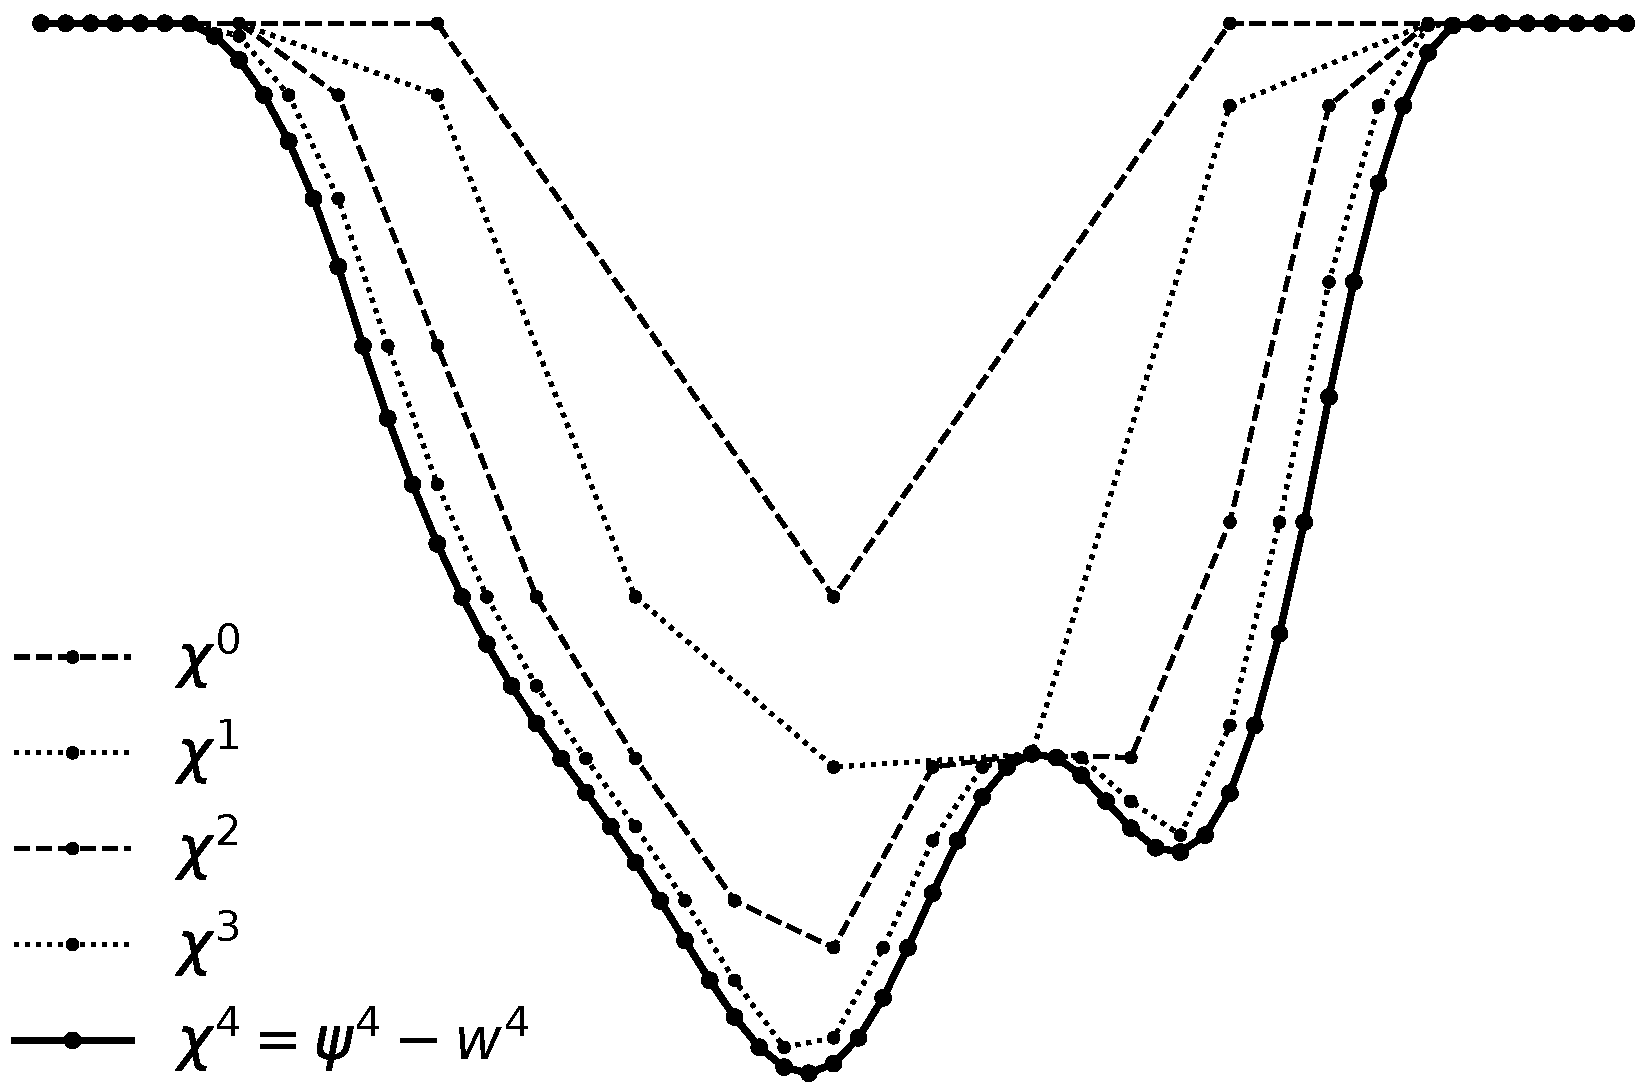
\includegraphics[width=0.55\textwidth]{fixfigs/chiphilevels.pdf}
\caption{Defect constraint $\chi^J = \gamma^J - w^J$ is decomposed using monotone restriction.}
\label{fig:chiphilevels}
\end{figure}

For the downward part of the multigrid V-cycle we will use the $\phi^j$ as constraints, and for the upward part the $\chi^j$.  That is, let
\begin{equation}
\mathcal{D}^j = \{v \in \mathcal{V}^j \,:\, v\ge \phi^j\}, \qquad \mathcal{U}^j = \{v \in \mathcal{V}^j \,:\, v\ge \chi^j\} \label{eq:fe:constraintsets}
\end{equation}
define \emph{downward} and \emph{upward constraint subsets} of the FE subspaces $\mathcal{V}^j$, respectively.  The upward sets are larger, $\mathcal{D}^j \subset \mathcal{U}^j$, and set decompositions $\mathcal{U}^j = \sum_{i=0}^j \mathcal{D}^i$ apply in the same sense as \eqref{eq:constraintdecomp}.

Returning to the central MCD idea, we will correct the finest-level iterate $w^J\in \mathcal{K}^J$ by adding modifications from each coarser subspace $\mathcal{V}^j$.  By nesting \eqref{eq:fe:nestedspaces} these corrections live in the fine-level subspace $\mathcal{V}^J$, but the corrected iterate needs to be admissible as well.  The accumulated corrections, from the constraint subsets $\mathcal{D}^j$ and $\mathcal{U}^j$, over the whole multigrid V-cycle, compute a new iterate in $\mathcal{K}^J$.

In detail, suppose $y^{j+1} \in \mathcal{D}^{j+1}, \dots, y^J \in \mathcal{D}^J$ are already-computed corrections during the downward part of the V-cycle (Figure \ref{fig:nmcdvcycle}).  The so-far corrected iterate is admissible, namely $w^J + y^J + \dots + y^{j+1} \in \mathcal{K}^J$, because the sum of corrections is in the (finest) defect constraint set, i.e.~$y^J + \dots + y^{j+1} \in \mathcal{U}^J = \{v\ge \chi^J\}$.

\begin{figure}[h]
\begin{center}
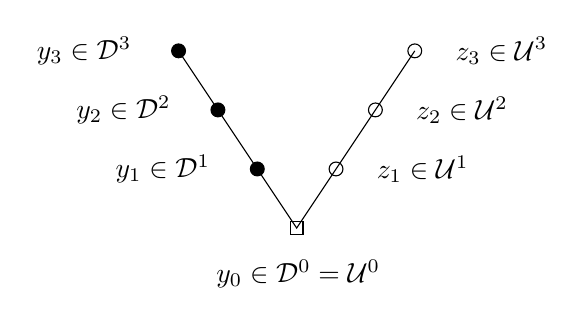
\begin{tikzpicture}[scale=1.0]
  \pgfmathsetmacro\hstep{0.5}
  \pgfmathsetmacro\vstep{0.75}
  \pgfmathsetmacro\ceps{0.08}   % size of square for coarse grid

% V-cycle with MCD down-obstacle and up-obstacle annotations
  \draw[black,thin] (-\hstep,3*\vstep) -- (0.0,2*\vstep) -- (\hstep,\vstep) --  (2*\hstep,0.0)
                    -- (3*\hstep,\vstep) -- (4*\hstep,2*\vstep) -- (5*\hstep,3*\vstep);
  \filldraw (-\hstep,3*\vstep) node[xshift=-12mm] {$y_3 \in \mathcal{D}^3$} circle (2.5pt);
  \filldraw (0.0,2*\vstep) node[xshift=-12mm] {$y_2 \in \mathcal{D}^2$} circle (2.5pt);
  \filldraw (\hstep,\vstep) node[xshift=-12mm] {$y_1 \in \mathcal{D}^1$} circle (2.5pt);
  \draw     (2*\hstep-\ceps,-\ceps) node[xshift=1mm,yshift=-5mm] {$y_0 \in \mathcal{D}^0 = \mathcal{U}^0$} rectangle (2*\hstep+\ceps,+\ceps);
  \draw     (3*\hstep,\vstep) node[xshift=11mm] {$z_1 \in \mathcal{U}^1$} circle (2.5pt);
  \draw     (4*\hstep,2*\vstep) node[xshift=11mm] {$z_2 \in \mathcal{U}^2$} circle (2.5pt);
  \draw     (5*\hstep,3*\vstep) node[xshift=11mm] {$z_3 \in \mathcal{U}^3$} circle (2.5pt);
\end{tikzpicture}

\end{center}
\caption{An NMCD V-cycle computes downward corrections $y_j \in \mathcal{D}^j$, but the upward corrections $z_j$ expand into larger constraint subsets $\mathcal{U}^j$.}
\label{fig:nmcdvcycle}
\end{figure}

When computing the next-coarser correction one must use the coarser-mesh representation of the problem.  As in nonlinear FAS multigrid schemes \cite{BrandtLivne2011,Bruneetal2015,Trottenbergetal2001}, this requires that we coarsen the iterate as well as the residual and the correction, and here injection is used \cite[section 5.3]{Trottenbergetal2001}.  Define
\begin{equation}
g^j = \begin{cases} w^J, & j=J \\
                    \iR(g^{j+1} + y^{j+1}), & j < J.
      \end{cases}  \label{eq:fe:defineg}
\end{equation}
Function $g^j$ is the $j$th-level mesh approximation to the solution of \eqref{eq:fe:vi}, before smoothing and correction at that level.\footnote{If we were to inject the finest-mesh obstacle downward to coarser meshes, $\gamma^{j-1} = \iR \gamma^j$, then, because $\iR$ preserves inequalities and $y^j \in \mathcal{D}^j$, it would follow that $g^j \ge \gamma^j$.  In this sense $g^j$ is admissible on the $j$th-level mesh.  However, following \cite{GraeserKornhuber2009}, our use of defect constraints $\chi^j$ avoids the need to generate the $\gamma^j$.}

Down-smoothing makes progress toward solving the following VI for $y^j \in \mathcal{D}^j$:
\begin{equation}
\ip{f^j(g^j + y^j)}{v-y^j} \ge \ip{\ell^j}{v-y^j} \qquad \text{for all } v\in \mathcal{D}^j. \label{eq:fe:downvi}
\end{equation}
Here $f^j$ is a discretization of $f$ in \eqref{eq:vi},\footnote{Again we diverge from the algorithm by Tai \cite{Tai2003}, who essentially assumes that ``$f(g^j + y^j)$'' is used here.  If $f$ is linear then efficient implementation via that formula is possible, but otherwise one must apply $f^j$.} using quadrature etc.~as addressed for $f^J$ in \eqref{eq:fe:vi}.

For $j<J$ the source function $\ell^j$ is determined by an FAS-type formula, as follows.  First note that the $j+1$ level version of \eqref{eq:fe:downvi} is not solved exactly by the correction $y^{j+1}$.  Fixing $y^{j+1} \in \mathcal{D}^{j+1}$, we would want to find a further correction $y$ so that $g^{j+1}+y^{j+1}+y$ is still admissible, and so that
\begin{equation}
\ip{f^{j+1}(g^{j+1}+y^{j+1}+y)}{v-y^{j+1}-y} \ge \ip{\ell^{j+1}}{v-y^{j+1}-y} \qquad \text{\emph{(notional)}} \label{eq:fe:downvinotional}
\end{equation}
held exactly.  However, in a multilevel method we actually compute this next correction $y$ on the next-coarser level $j$.  To do this we modify the notional finer-level VI \eqref{eq:fe:downvinotional} in five steps which mimic the standard argument for the FAS correction equations for PDEs \cite{BrandtLivne2011,Trottenbergetal2001}:
\begin{enumerate}
\item group $v-y^{j+1}$ as a coarser-level test function $v\in \mathcal{D}^j$,
\item subtract the known $f^{j+1}(g^{j+1}+y^{j+1}) \in (\mathcal{V}^{j+1})'$ from both sides,
\item replace the residual $\ell^{j+1}-f^{j+1}(g^{j+1}+y^{j+1})$ by its restriction,
\item replace $g^{j+1}+y^{j+1}$ where it appears by its restriction,
\item and replace $f^{j+1}$ by its coarser rediscretization $f^j$ where it appears on the left.
\end{enumerate}
Steps \emph{(iii)}--\emph{(v)} are justified, as usual, by the assumption that the residual and the correction should be smooth as a result of the progress made by the smoother on the $j+1$ level.  These steps now yield the precise $j$th-level VI problem, in cluttered form but the same as \eqref{eq:fe:downvi}:
\begin{align}
&\ip{f^j\left(\iR(g^{j+1}+y^{j+1})+y^j\right)}{v-y^j} - \ip{f^j\left(\iR(g^{j+1}+y^{j+1})\right)}{v-y^j} \label{eq:fe:downvicluttered} \\
&\qquad \ge \ip{R\left(\ell^{j+1}-f^{j+1}(g^{j+1}+y^{j+1})\right)}{v-y^j} \notag
\end{align}

Thus we define $\ell^j \in (\mathcal{V}^j)'$ in \eqref{eq:fe:downvi} by the following recursive definition, starting from $\ell^J$ already defined for the finest-level problem \eqref{eq:fe:vi}, and incorporating definition \eqref{eq:fe:defineg}:
\begin{equation}
\ell^j = f^j(g^j) + R\left(\ell^{j+1}-f^{j+1}(g^{j+1}+y^{j+1})\right). \label{eq:fe:levelsource}
\end{equation}
This is identical, even if the notation differs, to the standard FAS formula for a PDE source term, for example equation (8.5b) in \cite{BrandtLivne2011} or equation (5.3.14) in \cite{Trottenbergetal2001}.

At each level in the downward part of the V-cycle (Figure \ref{fig:nmcdvcycle}) we apply a smoother, a partial solver of \eqref{eq:fe:downvi} which should rapidly reduce the high-frequencies in the error, to generate a correction $y^j \in \mathcal{D}^j$.  At the coarsest $j=0$ level we solve \eqref{eq:fe:downvi}, accurately if possible, yielding a correction $y^0$ in the coarsest defect constraint set $\mathcal{D}^0=\mathcal{U}^0 = \{v \ge \chi^0\}$.  Note that the coarsest-level solver may be the same as the other smoothers.

In the upward part of the V-cycle the smoother starts from an initial iterate $z_0^j$ which has accumulated the coarser-level corrections.  Define $z_0^0 = y^0$ and
\begin{equation}
z_0^j = P z_0^{j-1} + y^j  \label{eq:fe:upwardaccumulation}
\end{equation}
where $P$ is canonical prolongation; stated simply, $z_0^j = y^j + \dots + y^0$.  By the decompositions $\mathcal{U}^j = \sum_{i=0}^j \mathcal{D}^i$, noted earlier, $z_0^j \in \mathcal{U}^j$.  This initial $z_0^j$ is smoothed to generate a result $z^j \in \mathcal{U}^j$ which approximately solves the same VI as the downward version \eqref{eq:fe:downvi}, except now we can solver over a larger set:
\begin{equation}
\ip{f^j(g^j + z^j)}{v-z^j} \ge \ip{\ell^j}{v-z^j} \qquad \text{for all } v\in \mathcal{U}^j. \label{eq:fe:upvi}
\end{equation}
The reason we can solve over $\mathcal{U}^j$, unlike during the downward phase, is that there is no forthcoming coarser correction which could violate admissibility.

These ideas come together in Algorithm \ref{alg:nmcd}, an NMCD V-cycle.  This procedure acts in-place on the final argument $w^J$, but it leaves the other inputs $\ell^J,\gamma^J$ unchanged.

\begin{pseudofloat}[H]
\begin{pseudo} \label{ps:nmcd-vcycle}
\pr{nmcd-vcycle}(\ell^J,\gamma^J;w^J)\text{:} \\+
    $\chi^J = \gamma^J - w^J$ \\
    $g^J = w^J$ \\
    for $j=J$ downto $j=1$ \\+
      $\chi^{j-1} = \mR \chi^j$ \\
      $\phi^j = \chi^j - P\chi^{j-1}$ \\
      $y^j = 0$ \\
      $\text{\pr{smooth}}^{\text{\id{down}}}(\ell^j,\phi^j,g^j;y^j)$  \ct{smoothing of \eqref{eq:fe:downvi} in $\mathcal{D}^j$}\\
      $g^{j-1} = \iR(g^j + y^j)$ \\
      $\ell^{j-1} = f^{j-1}(g^{j-1}) + R \left(\ell^j - f^j(g^j+y^j)\right)$ \\-
    $y^0 = 0$ \\
    $\text{\pr{solve}}(\ell^0,\chi^0,g^0;y^0)$ \ct{solving of \eqref{eq:fe:downvi} in $\mathcal{D}^0=\mathcal{U}^0$} \\
    $z^0 = y^0$ \\
    for $j=1$ to $j=J$ \\+
      $z^j = P z^{j-1} + y^{j}$ \\
      $\text{\pr{smooth}}^{\text{\id{up}}}(\ell^j,\chi^j,g^j;z^j)$  \ct{smoothing of \eqref{eq:fe:upvi} in $\mathcal{U}^j$} \\-
    $w^J \gets w^J+z^J$
\end{pseudo}
\caption{Nonlinear multilevel constraint decomposition V-cycle for the finest-level VI problem \eqref{eq:fe:vi}, as an in-place method on $w^J$, using mesh-level discretizations $f^j$ of the original nonlinear $f$ in problem \eqref{eq:vi}.}
\label{alg:nmcd}
\end{pseudofloat}

During one application of \pr{nmcd-vcycle}, storage must be allocated for $\chi^j$, $\phi^j$, $g^j$, $y^j$, and $\ell^j$ on each level.  However, line 3 is essentially notational in that the finest-level iterate $g^J$ is the same as $w^J$; no copy is needed.  Similarly, in algorithm lines 13 and 15 no allocation is required because the $y^j$ space can be reused for $z^j$ as the coarser corrections are prolonged and accumulated.  Let $m^j$ be the number of interior nodes in the $j$th-level mesh.  The total storage of \pr{nmcd-vcycle}, excluding any in the smoothers/solver, but including for the original obstacle $\gamma^J$, is about $8 m^J$ real numbers\footnote{That is: $8\approx 5(4/3) + 1$.} under the standard estimate that a 2D, uniform-mesh V-cycle uses $4/3$ the memory of the finest level alone \cite[Section 2.4]{Trottenbergetal2001}.  For comparison, a single-level method needs at least $3 m^J$ storage for the vectors $\ell^J,\gamma^J,w^J$.

\pr{nmcd-vcycle} assumes certain semantics for the smoothers and the coarsest-level solver; the latter might also be a smoother algorithm.  They do in-place modifications of their final arguments, and they do not modify their first three arguments.  The smoothers are in-exact solvers of VIs \eqref{eq:fe:downvi} and \eqref{eq:fe:upvi}, respectively, and they are iterated \id{down} and \id{up} times.  Further smoother implementation details and choices are addressed in the next section.

Repeated application of \pr{nmcd-vcycle} to solve VI \eqref{eq:fe:vi} will not reduce the finest-level residual $f^J(u^J) - \ell^J$ to zero everywhere.  However, recalling that a finite-dimensional VI is equivalent to a \emph{nonlinear complementarity problem} (NCP) \cite{FacchineiPang2003}, \eqref{eq:fe:vi} corresponds to the NCP
\begin{equation}
u^J \ge \gamma^J, \qquad f^J(u^J) \ge \ell^J, \qquad (u^J - \gamma^J)\left(f^J(u^J) - \ell^J\right) = 0.  \label{eq:fe:ncp}
\end{equation}
Thus, at convergence we only expect $f^J(u^J) = \ell^J$ at those locations where the constraint is inactive, namely where $u^J > \gamma^J$.  Therefore, recalling that the hat function at node $x_q^J$ is denoted $\psi_q^J$, for $w^J \in \mathcal{K}^J$ we define the following vector in $\RR^{m^J}$ as the finest-level \emph{nodal residual}:
\begin{equation}
\hat r(w^J)_q = \begin{cases} \ip{f^J(w^J)-\ell^J}{\psi_q^J}, & w^J(x_q^J) > \gamma^J(x_q^J), \\
                                  \min\{\ip{f^J(w^J)-\ell^J}{\psi_q^J},0\}, & w^J(x_q^J) = \gamma^J(x_q^J). \end{cases} \label{eq:cpresidual}
\end{equation}
(Formally, $\hat r:\mathcal{V}^J \to \RR^{m^J}$ is a nonlinear map.)  Observe that $\hat r(w^J)$ is nonzero if there are nodes where the NCP \eqref{eq:fe:ncp} is violated, either because $f^J(w^J)-\ell^J$ remains nonzero on the inactive set or because the same quantity is negative on the active set, and that nodal values of $f^J(w^J)-\ell^J$ are in evaluated in a weak sense, by application to a hat function.

A solver for \eqref{eq:fe:vi} using repeated applications of \pr{nmcd-vcycle} would start with an initial iterate $w^{J,0}$, do V-cycles, and stop once the finest-level nodal residual $\hat r(w^J)$ was sufficiently small.  For example, using tolerances \id{atol}$>0$ and \id{rtol}$>0$ the stopping criterion might be
\begin{equation}
\|\hat r(w^J)\| < \id{atol} \qquad \text{or} \qquad \frac{\|\hat r(w^J)\|}{\|\hat r(w^{J,0})\|} < \id{rtol},
\end{equation}
where $\|\cdot\|$ denotes a norm on $\RR^{m^J}$.  A step tolerance could also be used, measuring the difference between successive iterates.

FIXME in Appendix we show how NMCD reduces to FAS if the obstacle is removed and to MCD if $f$ is assumed to be linear



\section{Smoother implementations} \label{sec:smoothers}

FIXME

Recall that a $j$th-level hat function based at node $x_p^j$ is denoted $\psi_p^j$, for an iterate $g^j$ and an admissible correction $y^j \in \mathcal{D}^j$ we define the \emph{downward nodal residual} as
\begin{equation}
(\hat r_{\text{down}}(y^j))_p = \begin{cases} \ip{f^j(g^j+y^j)-\ell^j}{\psi_p^j}, & y^j(x_p^j) > \phi^j(x_p^j), \\
                                  \min\{\ip{f^j(g^j+y^j)-\ell^j}{\psi_p^j},0\}, & y^j(x_p^j) = \phi^j(x_p^j). \end{cases} \label{eq:cpresidual}
\end{equation}
The \emph{upward nodal residual} $\hat r_{\text{up}}(z^j)$ for $z^j \in \mathcal{U}^j$ is similarly defined using $\chi^j$.

FIXME stopping criteria for smoother


\section{Results} \label{sec:results}

FIXME show results for 2D Firedrake implementation of NMCD for $p$-Laplacian obstacle problem (Example \ref{ex:plaplacian}), advection-diffusion obstacle problem (Example \ref{ex:advectiondiffusion}), and porous-media obstacle problem (Example \ref{ex:porous})

FIXME observe that up-smoothing is more efficient

% A BRIDGE TOO FAR:  \section{Results for a nonlocal variational inequality}


\bibliography{mcd2}
\bibliographystyle{siam}

\appendix
\section{Reductions of the NMCD algorithm}

FIXME by removing obstacle, reduce to ordinary FAS as in \cite{Bruneetal2015}

FIXME by assuming $N$ is linear, reduce to Algorithm 4.7 in \cite{GraeserKornhuber2009} but with $\text{V}(\nu_1,\nu_2)$ cycles which works for linear

\end{document}

